%---------------------------------------------------------------------------
% Gui component.
%
%---------------------------------------------------------------------------
\section{GUI component}
\label{sec:arch_gui}

Graphical user interfaces are most commonly used form of interaction with user in modern computing. Designing decent user interface is especially significant due to aim of this work - creation of measurement and visualization tool. Although GUI component has rather limited role of giving the user control over application and allowing viewing results of the work, in fact, it is the most complex component. Additionally, any shortcoming in GUI is relatively difficult to hide from the user. It makes UI/UX (User Interface/User Experience) engineering valuable.

While designing the user interface, I've been trying to follow few general principles. First of all, I wanted to result interface to be as transparent as possible. Users should focus on their tasks instead of learning how to use the tool. Because of that, application should not be bloated with unnecessary options and steps that need to be performed by users need to achieve their goals should be as short as possible. Because measurement visualization is probably most essential functionality of application, it needs significant concern. User should be able to view charts with results without any interruptions or any other UI components that might be disturbing. What is also noteworthy, GUI must be coherent to free user from chaos of being spread across multiple windows, desktops.

From business logic point of view, GUI component will extensively use MVC design pattern\cite{gamma1995}. Each form, window or more complex section needs to have its own View, responsible for presentation, Controller that collects user's events and updates view on user actions or system events. Application will use shared model, which will be an access point for underlying, external to GUI components.

\subsection{Interface Mockups}

In this section, I will try to describe mockups of most fundamental views. First one, depicted in Figure~\ref{fig:mock_main} shows main application view. Left edge of the application window contains vertical tab pane controller that will allow the user easily to switch views covering most notable application contexts - resources, measurements and visualizations. Another benefit of such an approach is that the application has a lot of space for what user needs. The second most vital component of the main view is a menu bar placed on top. It allows a user to perform bulk operations (e.g. pause all measurements) regardless of view that a user currently sees.

All subsequent mockups cover context-specific views that applications renders in central pane of the main view.

\begin{figure}[ht]
\centering
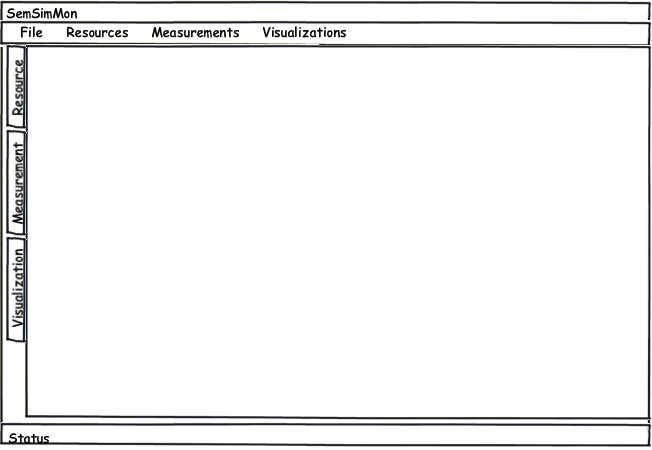
\includegraphics[width=0.7\textwidth]{mock_main}
\caption{GUI application main view mockup}
\label{fig:mock_main}
\end{figure}

When user starts working with application, He or She must first add resources to measure. Because of that the resources view is the first, initial section displayed directly after a startup. Resources Mockup can be found in Figure~\ref{fig:mock_resources}. The view is divided into two high level logical parts - the left pane covers global resources context - users can browse measurement tree as well as add new resources into it. The right pane is specific to resource selected by user from tree on left and contains accordion with two sections. The upper one shows resource\rq{}s static attributes. The one below allows a user to see snapshot of its dynamic state and check all of its capabilities at given point of time. It contains also the Refresh button, to allow the user to refresh those values. Additionally, below accordion there are several buttons allowing performing actions on selected resource.

\begin{figure}[ht]
\centering
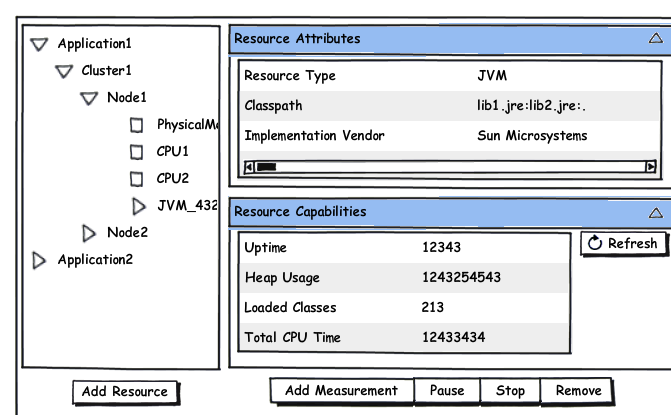
\includegraphics[width=0.7\textwidth]{mock_resources}
\caption{GUI application resources pane}
\label{fig:mock_resources}
\end{figure}

Figure~\ref{fig:mock_measurements} covers the measurements context of the application. All measurements created are listed on the left side of this view. Accordion on the right side shows details of selected measurement after selecting one of them. The upper section contains a table with general information. The lower one shows all values gathered since the creation of selected resource. Using controls under measurements list, user can pause, resume or remove measurement. Additionally in this section user may copy the results to clipboard, in CSV format which can be easily imported to any spreadsheet application for further analysis.

\begin{figure}[ht]
\centering
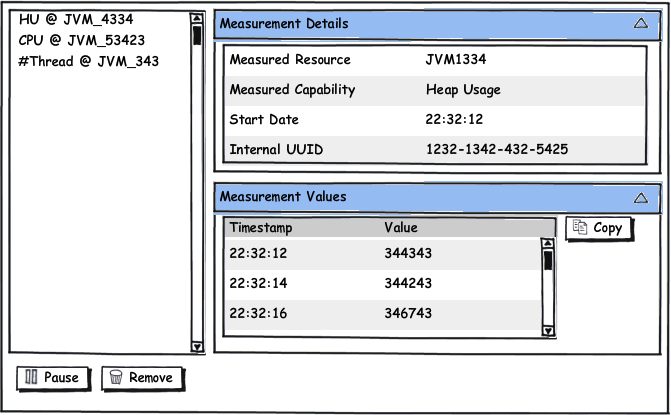
\includegraphics[width=0.7\textwidth]{mock_measurements}
\caption{GUI application measurements pane}
\label{fig:mock_measurements}
\end{figure}

\begin{figure}[ht]
\centering
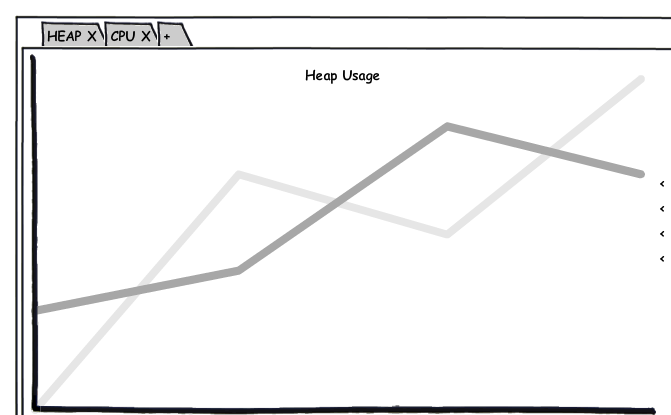
\includegraphics[width=0.7\textwidth]{mock_vis_clean}
\caption{GUI application visualizations pane, clean view}
\label{fig:mock_vis_clean}
\end{figure}

Appropriate visualizations display is probably most difficult to design from user experience engineering perspective. I have been using modest web browsers interfaces as an inspiration during designing this UI component. The effects can be seen in Figure~\ref{fig:mock_vis_clean} - in proposed solution every visualization is being rendered on separate, horizontal tab. The user should just click last tab with prompting icon to add new visualization. To remove visualization - user simply clicks cross icon on visualization tab - just as He or She would close tab in a browser. This gives visualization chart as much space as possible and still allows the user to control creation easily and disposal of visualization.

Where to place controls of visualization is the biggest problem with such an approach. The user must be able to choose which measurements should be included in given visualization, as well as chart type or define other configuration settings. A management pane was designed to address this need. It is hidden by default and is being displayed to the user, on mouse over the right edge of chart, marked with \lq{}<\rq{} signs. Figure~\ref{fig:mock_vis_options} depicts layout of this pane. The settings pane contains form, divided into several sections:

\begin{itemize}

\item Visualization Options - here user can configure a label of a whole visualization, as can be seen on a tab pane

\item Chart Options - allows setting a chart title (the rendered on chart graphics pane) and choose a type of the chart. The user will be able to use a line (XY scatter), a pie, a bar and a spider web chart types.

\item Measurements - gives control over which measurements should be included in given visualization. To add a measurement into a visualization, user should click the Add button and choose which measurements should be included from a displayed dialog. System doesn't give any constraints on measurements to be chosen, so it is up to the user to prepare a reasonable visualization. The user will be able to remove given measurement from a chart, by simply selecting it from the list and clicking Remove button.

\item Actions - allows user to pause and resume the visualization. Additionally the user can copy to clipboard an image containing snapshot of the visualization's chart.
\end{itemize}

\begin{figure}[ht]
\centering
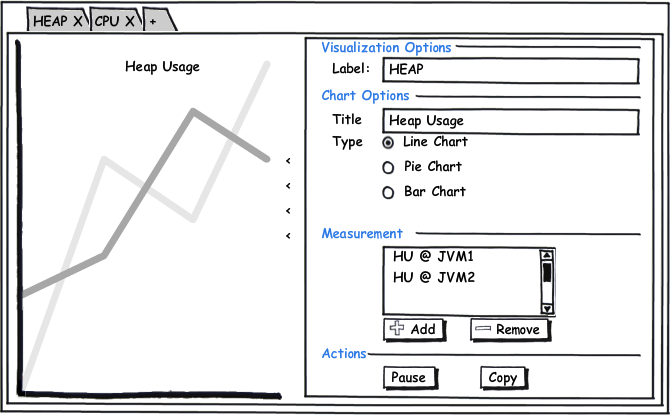
\includegraphics[width=0.7\textwidth]{mock_vis_options}
\caption{GUI application visualizations pane, view with options pane}
\label{fig:mock_vis_options}
\end{figure}

